%% LaTeX Beamer presentation template (requires beamer package)
%% see http://bitbucket.org/rivanvx/beamer/wiki/Home
%% idea contributed by H. Turgut Uyar
%% template based on a template by Till Tantau
%% this template is still evolving - it might differ in future releases!

\documentclass[brazil]{beamer}

\mode<presentation>
{
%\usetheme{Hannover}
%\usetheme{Hannover}
\usetheme{LRM}

%\usetheme{PaloAlto}
%\usetheme{Madrid}
%\usetheme{Szeged}
%\usetheme{Ilmenau}
%\usetheme{Sanca}
%\usetheme{CambridgeUS}
%\usecolortheme{wolverine}
%\usetheme{progressbar}
%\usecolortheme{crane}
\setbeamercovered{transparent}
%\progressbaroptions{}

\setbeamertemplate{footline}[page number]
%%\setbeamertemplate{headline}[page number]
}


\usepackage[brazil]{babel}
%\usepackage[latin1]{inputenc}
\usepackage[utf8]{inputenc}

% font definitions, try \usepackage{ae} instead of the following
% three lines if you don't like this look
\usepackage{mathptmx}
\usepackage[scaled=.90]{helvet}
\usepackage{courier}
\usepackage[T1]{fontenc}

\title[Projeto de Mestrado]{
Navegação de Veículos Autônomos em Ambientes Externos 
Não Estruturados Baseada em Visão Computacional}


% - Use the \inst{?} command only if the authors have different
%   affiliation.
%\author{F.~Author\inst{1} \and S.~Another\inst{2}}
\author[Rafael Luiz Klaser]{Rafael Luiz Klaser \\
Orientador: Prof. Dr. Fernando Santos Osório}

% - Use the \inst command only if there are several affiliations.
% - Keep it simple, no one is interested in your street address.
\institute[ICMC - USP São Carlos]
{
Laboratório de Robótica Móvel\\

\includegraphics[width=2cm,height=1cm,clip=true]{icmc.png}
}

\date{Outubro 2012}

%\bibliography{bibtex}

\bibliography{quali}

\begin{document}

\begin{frame}
\titlepage

\includegraphics[width=2cm,height=0.5cm,clip=true]{fapesp.jpg}
\textit{\tiny Apoio \#2012/04555-4}
\end{frame}


\begin{frame}
\frametitle{Sumário}
\framesubtitle{roteiro da apresentação}
\tableofcontents
\end{frame}


\section{Resumo da Introdução}

\subsection[Objetivo]{Objetivo}


\begin{frame}
\frametitle{Resumo da Introdução}
\framesubtitle{Objetivo}
Desenvolver um método de navegação autônoma, deliberativo, focado em ambientes
externos não estruturados, com base em um mapa de navegabilidade com informação
espacial (tridimensional) construído a partir de visão estéreo.
\end{frame}

\subsection[Contribuições]{Contribuições Esperadas}

\begin{frame}
\frametitle{Resumo da Introdução}
\framesubtitle{Contribuições}
% Contribuição para a percepção espacial em métodos de navegação autônoma de
% robôs terrestres,
\begin{itemize}
\item Aperfeiçoamento de algoritmos de geração de mapas de disparidade e nuvem de pontos;
\item Proposta e desenvolvimento de algoritmo para a obtenção de mapas locais de 
navegabilidade com informações espaciais (3D);
\item Aperfeiçoamento de técnicas para a navegação baseada no uso de GPS, 
bússola e mapas locais de navegabilidade (onde as pesquisas previamente 
desenvolvidas para detectar e desviar de obstáculos com o uso de mapas 2D 
serão estendidas a fim de trabalhar com mapa de navegabilidade/ocupação em 3D).
\end{itemize}
\end{frame}


\subsection[Conceitos]{Conceitos Abordados}

\begin{frame}
\frametitle{Resumo da Introdução}
\framesubtitle{Conceitos abordados}
\begin{itemize}
\item Visão estéreo / Calibragem;
\item Mapas de disparidade;
\item Nuvens de pontos;
\item Segmentação / Representação espacial (Stixel, Octomap).
\end{itemize}
\end{frame}


\section{Proposta de Pesquisa}

\subsection[Tema]{Tema}


\begin{frame}
\frametitle{Proposta de Pesquisa}
\framesubtitle{Temas centrais}
\begin{itemize}
\item Visão estéreo
\item Mapas de navegabilidade a partir de informação tridimensional
\end{itemize}
\end{frame}


\begin{frame}
\frametitle{Proposta de Pesquisa}
\framesubtitle{Temas centrais - Propósitos}
\begin{block}{Visão estéreo}
Obter a informação espacial do ambiente
\end{block}
\end{frame}


\begin{frame}
\frametitle{Proposta de Pesquisa}
\framesubtitle{Temas centrais - Propósitos}
\begin{block}{Mapa de navegabilidade}
Para uma navegação deliberativa é necessário o planejamento da trajetória, para isso é necessário 
um mapa (local / global)
\end{block}
\end{frame}


\begin{frame}
\frametitle{Proposta de Pesquisa}
\framesubtitle{Planejamento de trajetória\ldots}
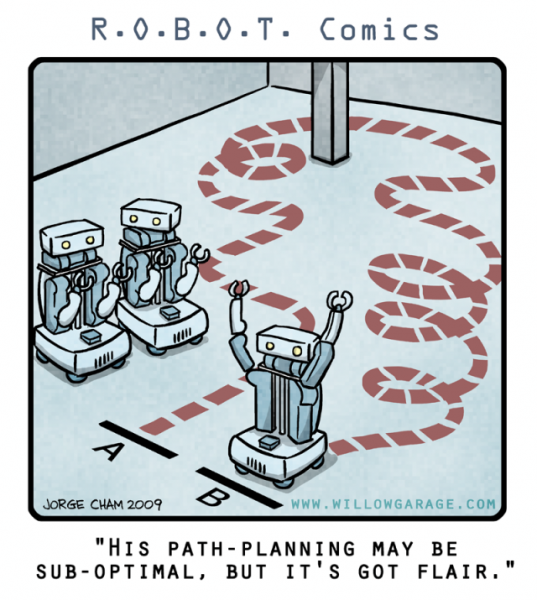
\includegraphics[width=10cm,height=7cm,]{nav_comic.png}
\end{frame}


\subsection[Discussão]{Discussão}


\begin{frame}
\frametitle{Proposta de Pesquisa}
\framesubtitle{Discussão - Visão Computacional}
\begin{block}{}
Apesar de uma das vantagens das câmeras de vídeo ser a geração de nuvens de pontos densas, 
uma abordagem que produza nuvens menos densas por quadro pode ser aplicada, tendo a densidade 
compensada no tempo (aumentando o desempenho geral sem grande perda da informação global);
\end{block}
\begin{block}{}
A informação global requer maior precisão apenas na trajetória a ser seguida, 
podendo ser aplicado conceito de \textit{foco de atenção};
\end{block}
\end{frame}

\begin{frame}
\frametitle{Proposta de Pesquisa}
\framesubtitle{Discussão - Visão Computacional}
\begin{block}{}
Na visão computacional pode-se identificar duas linhas de abordagem: 
a geométrica e a cognitiva;
\end{block}
\begin{block}{}
Abordagens cognitivas (associas a custo computacional elevado) já se tornam
praticáveis (computação em GPU) 
\footnote{Teste preliminar com geração de mapa de disparidade a partir do canal 
Magno-Celular se demonstrou promissor no conceito de mapas com densidade variável 
pelo foco de atenção} 
\end{block}
\end{frame}


\begin{frame}
\frametitle{Proposta de Pesquisa}
\framesubtitle{Em resumo - Visão Computacional}
\begin{block}{}
A proposta é buscar a geração de nuvens de pontos com a densidade nas regiões de maior
interesse na imagem. 
\end{block}
\end{frame}


\begin{frame}
\frametitle{Proposta de Pesquisa}
\framesubtitle{Discussão - Mapa de navegabilidade}
\begin{block}{}
%As abordagens de navegação por mapas planares assumem condições limitadas do ambiente  
%- geralmente ambiente interno e estruturado.
Um veículo terrestre se desloca na sua superfície de suporte (plano do chão), em condições controladas é
possível limitar-se à uma superfície planar.
\end{block}
\begin{block}{}
Para ambientes externos não estruturados existe maior necessidade da noção espacial 
do ambiente principalmente pela irregularidade do terreno, logo, a abordagem por mapas
que contenham essa noção é justificada. 
\end{block}
\end{frame}


\begin{frame}
\frametitle{Proposta de Pesquisa}
\framesubtitle{Discussão - Mapa de navegabilidade}
\begin{block}{}
Será utilizado o conceito de ocupação com probabilidade associada pois permite melhor atualização dos mapas.
\textit{Porém seria interessante classificar tais regiões e suas 
probabilidades também com possíveis elementos ``transponíveis'' - Trabalhos futuros.}
\end{block}
\begin{block}{}
Uma vegetação não é necessariamente um obstáculo bloqueante, podendo ser transponível (ex grama, capim);
\end{block}
\end{frame}


\begin{frame}
\frametitle{Proposta de Pesquisa}
\framesubtitle{Em resumo - Mapa de navegabilidade}
\begin{block}{}
A proposta é buscar uma representação em mapa suficiente para descrever o espaço de navegação
do veículo.
\end{block}
\begin{block}{}
Idealmente seria desejável uma representação semelhante a um mapa topográfico - Trabalhos futuros.
\end{block}
\end{frame}
\section{Materiais e Métodos}


\begin{frame}
\frametitle{Materiais e Métodos}
\framesubtitle{Equipamentos}
\begin{itemize}
\item Plataforma CaRINA I (veículo)
\item GPS + IMU (localização e odometria)
\item Câmeras de vídeo (binocular, trinocular, etc\ldots)
\end{itemize}
\end{frame}


\begin{frame}
\frametitle{Materiais e Métodos}
\framesubtitle{CaRINA I}
 CaRINA (Carro Robótico Inteligente para Navegação Autônoma)
\begin{columns}[c]
\begin{column}{5cm}
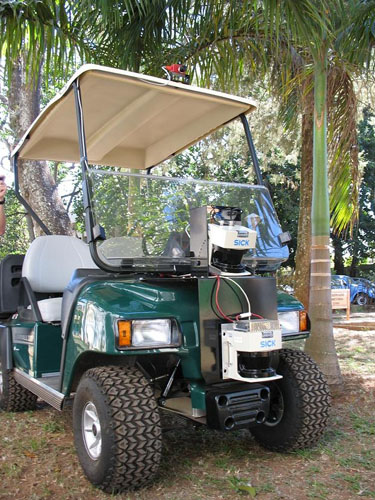
\includegraphics[width=5cm,keepaspectratio]{carina1_1.jpg}
\end{column}
\begin{column}{5cm}
\begin{itemize}
\item 
\includegraphics[width=1.5cm,keepaspectratio]{inct.jpg}
\item 
\includegraphics[width=1.5cm,keepaspectratio]{fapesp.jpg}
\item 
\includegraphics[width=1.5cm,keepaspectratio]{cnpq.png}
\end{itemize}
\end{column}
\end{columns}
\end{frame}


\begin{frame}
\frametitle{Materiais e Métodos}
\framesubtitle{Ferramentas}
\begin{itemize}
\item ROS (Robotic Operating System)
\item Gazebo - Simulação física (corpos rígidos)
\end{itemize}
\end{frame}


\begin{frame}
\frametitle{Materiais e Métodos}
\framesubtitle{ROS}
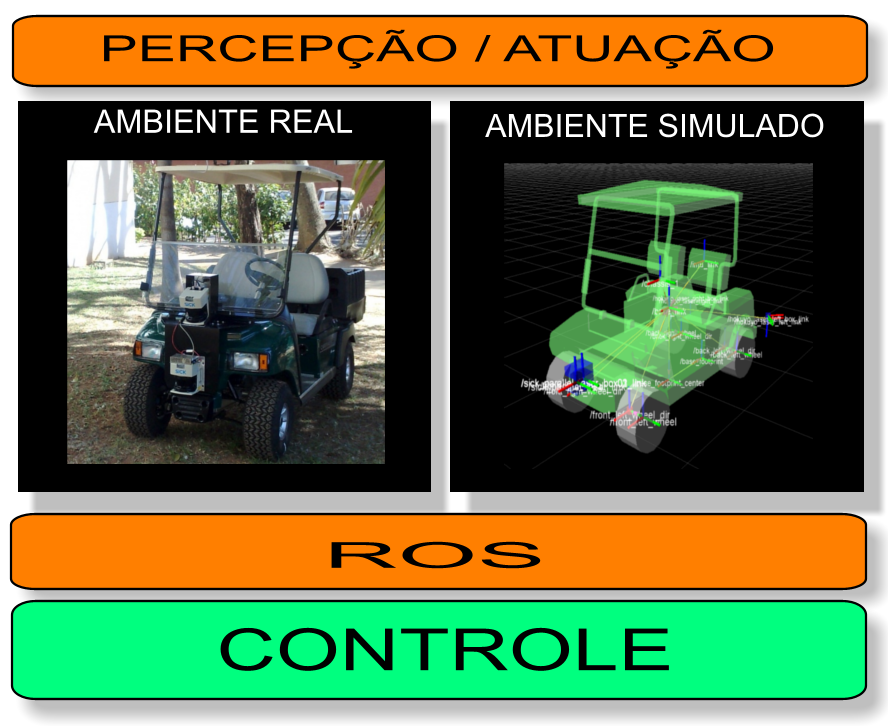
\includegraphics[width=9cm,keepaspectratio]{ros-slide.png}
\end{frame}


\begin{frame}
\frametitle{Materiais e Métodos}
\framesubtitle{ROS}
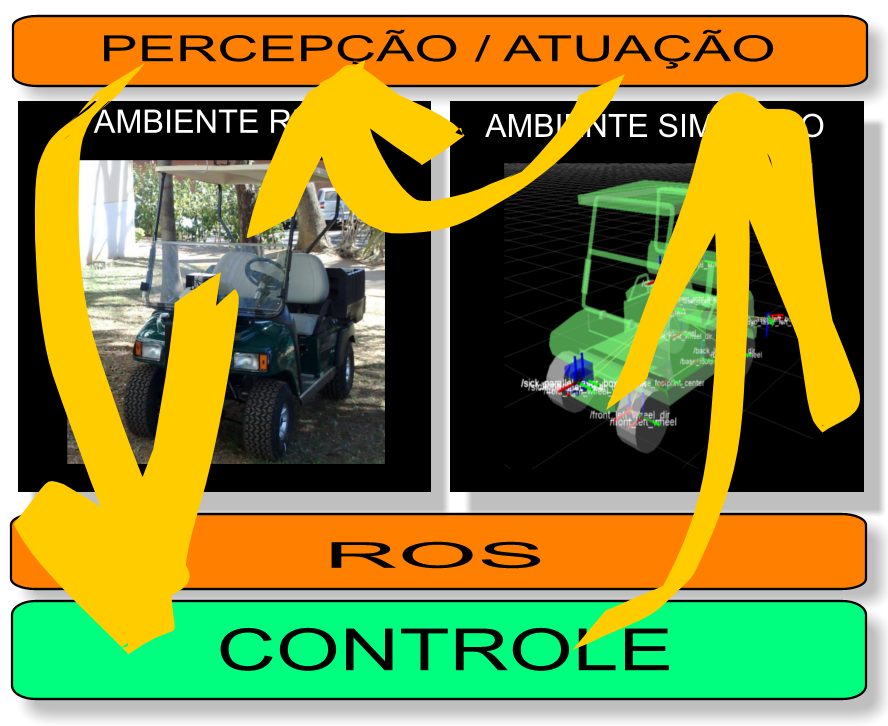
\includegraphics[width=9cm,keepaspectratio]{ciclo-rob.png}
\end{frame}


\begin{frame}
\frametitle{Materiais e Métodos}
\framesubtitle{ROS}
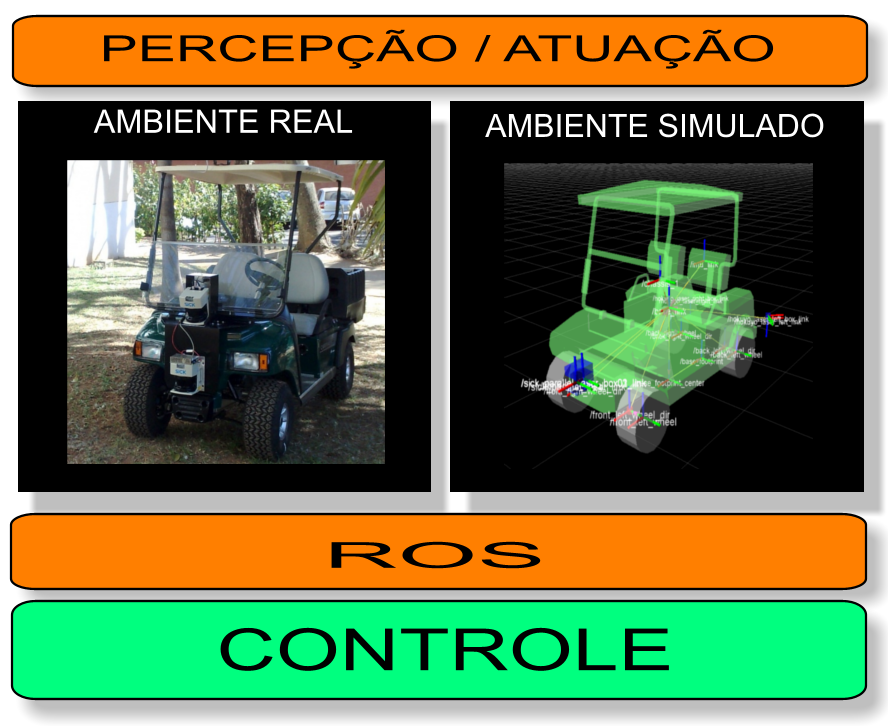
\includegraphics[width=9cm,keepaspectratio]{ros-slide.png}
\end{frame}


\begin{frame}
\frametitle{Materiais e Métodos}
\framesubtitle{Planejamento}
\begin{block}{De forma iterativa}
\begin{block}{}
\begin{itemize}
\item Coleta de dados (ambiente real)
\end{itemize}
\end{block}
\begin{block}{}
\begin{itemize}
\item Simulação e análise com os dados coletados
\item Verificação (comportamento) em ambiente simulado 
\end{itemize}
\end{block}
\begin{block}{}
\begin{itemize}
\item Validação (ambiente real)
\end{itemize}
\end{block}
\end{block}
\end{frame}


\begin{frame}
\frametitle{Materiais e Métodos}
\framesubtitle{Simulação}
\begin{block}{Vantagens}
\begin{itemize}
\item Maior repetibilidade dos experimentos
\item Replicação dos experimentos (e sem necessidade do equipamento físico)
\item Versatilidade
\end{itemize}
\end{block}
\begin{block}{Desvantagens}
\begin{itemize}
\item A modelagem dos cenários é custosa (tempo)
\item Não reflete fielmente a realidade
\end{itemize}
\end{block}
\end{frame}



\section{Cronograma}


\begin{frame}
\frametitle{Cronograma}
\framesubtitle{Macro Atividades}
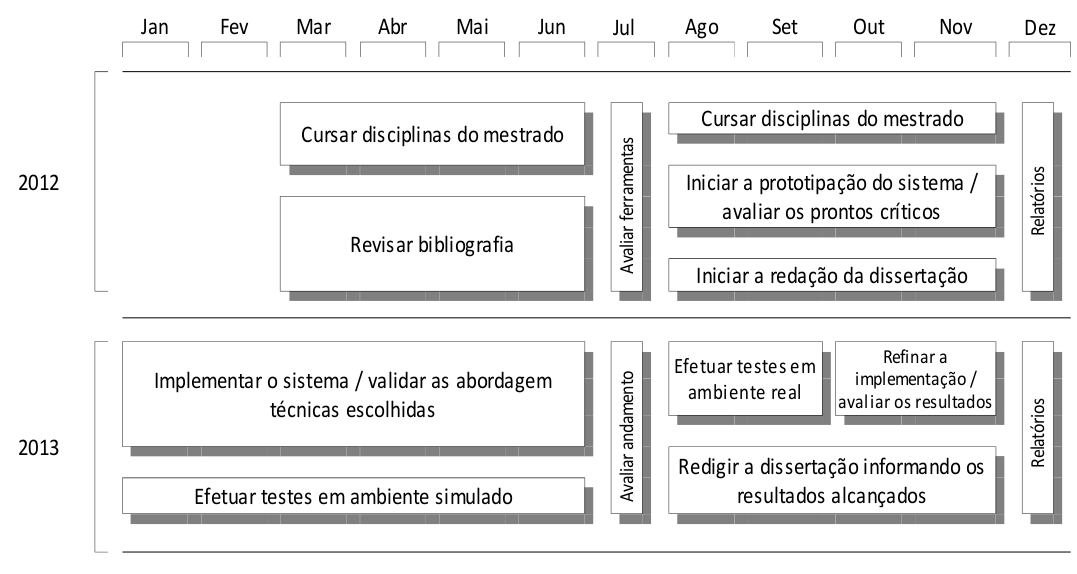
\includegraphics[width=10cm,height=7cm,]{chrono.png}
\end{frame}


\begin{frame}
\frametitle{Perguntas?}
\centering
\begin{columns}[t]
\begin{column}{4cm}

\includegraphics[width=3cm,keepaspectratio]{logo.png}
\end{column}
\begin{column}{4cm}

\includegraphics[width=3cm,keepaspectratio]{icmc.png}
\end{column}
\end{columns}
\end{frame}
\end{document}

